\chapter{\IfLanguageName{dutch}{Stand van zaken}{State of the art}}%
\label{ch:stand-van-zaken}

% Tip: Begin elk hoofdstuk met een paragraaf inleiding die beschrijft hoe
% dit hoofdstuk past binnen het geheel van de bachelorproef. Geef in het
% bijzonder aan wat de link is met het vorige en volgende hoofdstuk.

% Pas na deze inleidende paragraaf komt de eerste sectiehoofding.

In deze sectie van de paper wordt nagegaan wat voor onderzoek er al verricht is over het thesis onderwerp. Deze sectie begint met een korte beschrijving van het concept CI/CD en hoe DevOps daarin thuis hoort. Wanneer er gesproken wordt over het beveiligen van deze omgevingen, wordt er gebruik gemaakt van een nieuwe filosofie namelijk DevSecOps. In het tweede hoofdstuk van deze sectie wordt kort geschetst waar security thuishoort binnen deze filosofie. Om te onderzoeken hoe secrets binnen een Jenkins omgeving het best beschermd worden, is het ook belangrijk in kaart te brengen welke kwetsbaarheden bestaan binnen deze context. Het volgende hoofdstuk in deze sectie behandelt daarom bestaand onderzoek over deze kwetsbaarheden. In dit hoofdstuk word besproken welke aanvallen mogelijk zijn dankzij deze kwetsbaarheden en hoe deze aanvallen gebruikt kunnen worden om gevoelige informatie te extraheren uit de pipeline. Het laatste hoofdstuk van deze sectie wordt gebruikt om samen te vatten wat voor onderzoek er al verricht is over het beveiligen van de pipeline en het beveiligen van secrets voor een CI/CD oplossing.

\section{\IfLanguageName{dutch}{CICD en DevOps in kort}
{CICD and DevOps in brief}}
\label{sec:CICD em DevOps in kort}

De vraag naar sofware stijgt alleen maar en om aan deze vraag te kunnen voldoen is er nood aan automatisatie. Binnen de software wereld is er dus nood aan een aanpak waar de focus ligt op het automatiseren van software. DevOps is de tak binnen de IT die zich bezig houdt met deze aanpak. Het doel van DevOps is om sotwareontwikkeling te automatiseren en software-implementatie in productieomgevingen te integreren. Binnen deze filosifie wordt gebruik gemaakt van automatiseringstools en best practices om de snelheid, betrouwbaarheid en kwaliteit van de softwareontwikkeling te verbeteren.
\newline

Deze automatiseringstools worden gebruikt in de CI/CD pipeline. Het eerste deel van de CI/CD pipeline staat voor continue integratie. De code die geschreven wordt door developers ondergaat heel wat wijzigingen deze wijzigingen worden bijgehouden in een versiebeheer systeem. Continue integratie zorgt ervoor dat de code die gewijzigd wordt getest en gebouwd wordt.
\newline

het tweede deel van de pipeline bestaat uit twee processen continue levering and continue implementatie. Continue levering is de stap waarin de code voorbereid wordt om gedployed te worden in productie. Via de pipeline worden zoveel mogelijk aspecten getest zoals UI testing, integration testing, load testing, API reliability testing. Dankzij continue leverling is het mogelijk het leverlingsproces te automatiseren. Tegenwoordig wordt gebruik gemaakt van de cloud en cluster oplossingen om de sofware bij de klant te leveren.

\section{\IfLanguageName{dutch}{DevSecOps binnen de pipeline}{DevSecOps within the pipeline}}
\label{sec:DevSecOps binnen de pipeline}

\subsection{\IfLanguageName{dutch}{DevSecOps impact op de pipeline}{Devsecops impact on the pipeline}}
\label{sec:DevSecOps impact op de pipeline}
Om een beter beeld te schetsen over het gebruik van secrets, is het belangrijk de omgeving waarin deze gevoelige informatie gebruikt wordt, te analyseren. Binnen deze omgeving wordt vooral te werk gegaan volgens de DevOps mentaliteit. De DevOps aanpak bestaat reeds lange tijd maar deze voldoet niet meer aan de security vereisten die vandaag gesteld worden. Tegenwoordig is er steeds meer een verschuiving naar een andere filosofie, de DevSecOps filosofie. DevSecOps zorgt ervoor dat beveiliging in de pipeline geïntegreerd wordt. Op die manier wordt de beveiliging niet alleen toegepast op het afgewerkte product, maar zit de beveiliging ingebouwd in het product zelf. Deze beveiling is voorzien binnen elke fase van de typische DevOps pipeline. Elk DevOps team is dan ook verantwoordelijk voor het volgen van de best practices om een veilige pipeline te garanderen.\autocite{Zettler2020}
\newline

Een bedrijf kan niet van de ene op de andere dag DevSecOps implementeren. Om deze filosofie te integreren in de moderne software development levenscyclus (SDLC), is er nood aan een strategie \autocite{Jenkins2021}. \textcite{Ahmed2019} beschrijft in zijn master thesis welke invloed deze aanpak heeft op de SDLC. Het concept waar software pas getest wordt op veiligheidsrisico's na het ontwikkelen is niet genoeg om veilige software af te leveren aan de klant. Er moet al vanaf de design fase aandacht gegeven worden aan security en security moet vertegenwoordigd worden in elke fase van het development proces. Verder toont \textcite{Ahmed2019} aan met deze thesis dat wanneer deze aanpak correct geïmplementeerd wordt, development teams alleen maar sneller betere en vooral veiligere software kunnen opleveren. Security is dus eerder een katalysator die het development proces naar een hoger niveau tilt. 
In figuur \ref{fig:schema_DevSecOpsStrategie} is een voorbeeld te zien van hoe zo'n strategie er mogelijks kan uitzien.

\begin{figure}[H]
  \centering
  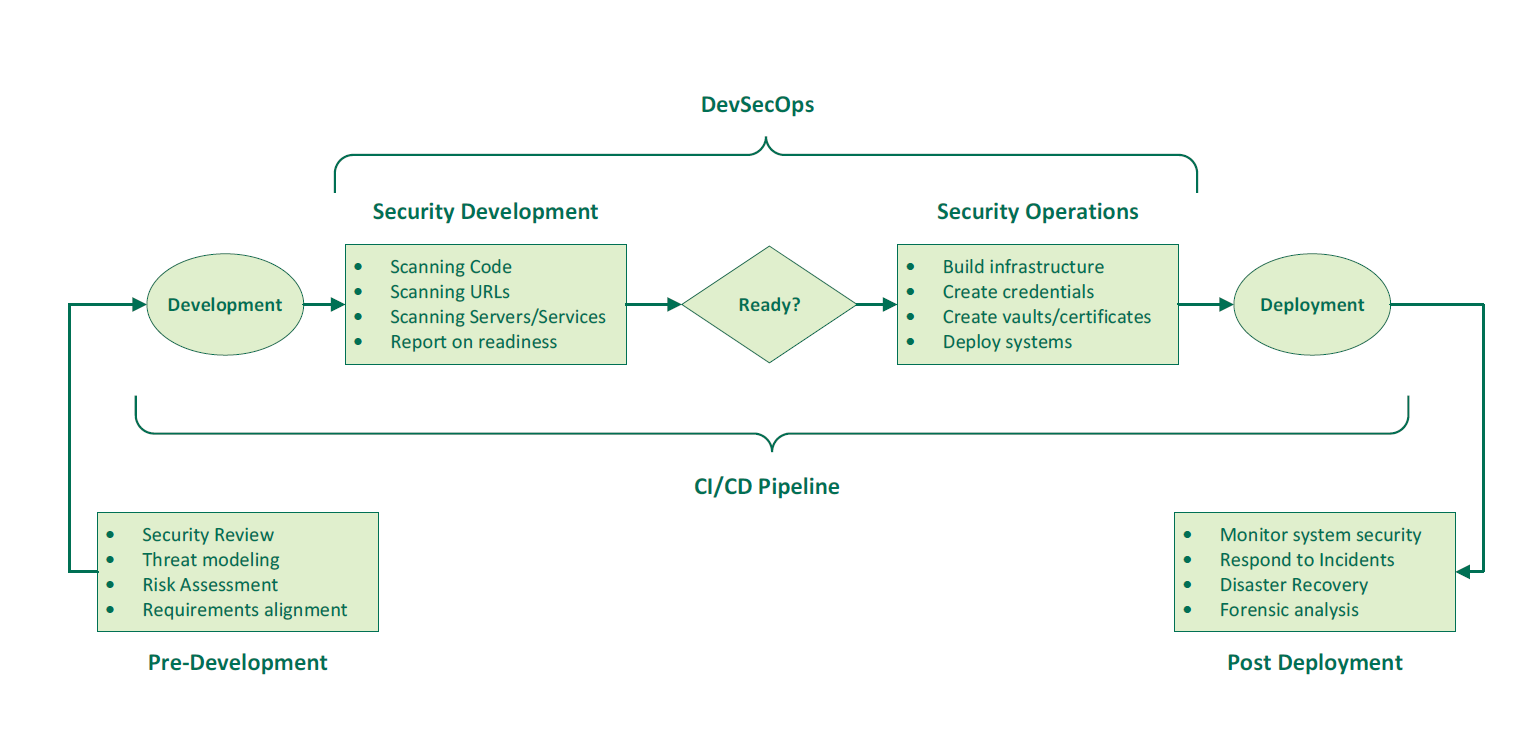
\includegraphics[scale=0.35]{graphics/schema_DevSecOpsStrategie.png}
  \caption{\label{fig:schema_DevSecOpsStrategie}Voorbeeld van een DevSecOps strategie binnen een CI/CD omgeving \autocite{Jenkins2021}.}
\end{figure}

\subsection{\IfLanguageName{dutch}{Het gebruik van security tools binnen DevSecOps}{Using security tools within DevSecOps}}
\label{sec:Het gebruik van security tools binnen DevSecOps}
Om secrets te beschermen in een CI/CD omgeving is er nood aan verschillende tools die ingezet kunnen worden in elke fase van het ontwikkelingsproces. Deze tools worden onderverdeeld in de volgende categorieën, deze zijn te zien in figuur \ref{fig:wordcloud}.

\begin{figure}[H]
  \centering
  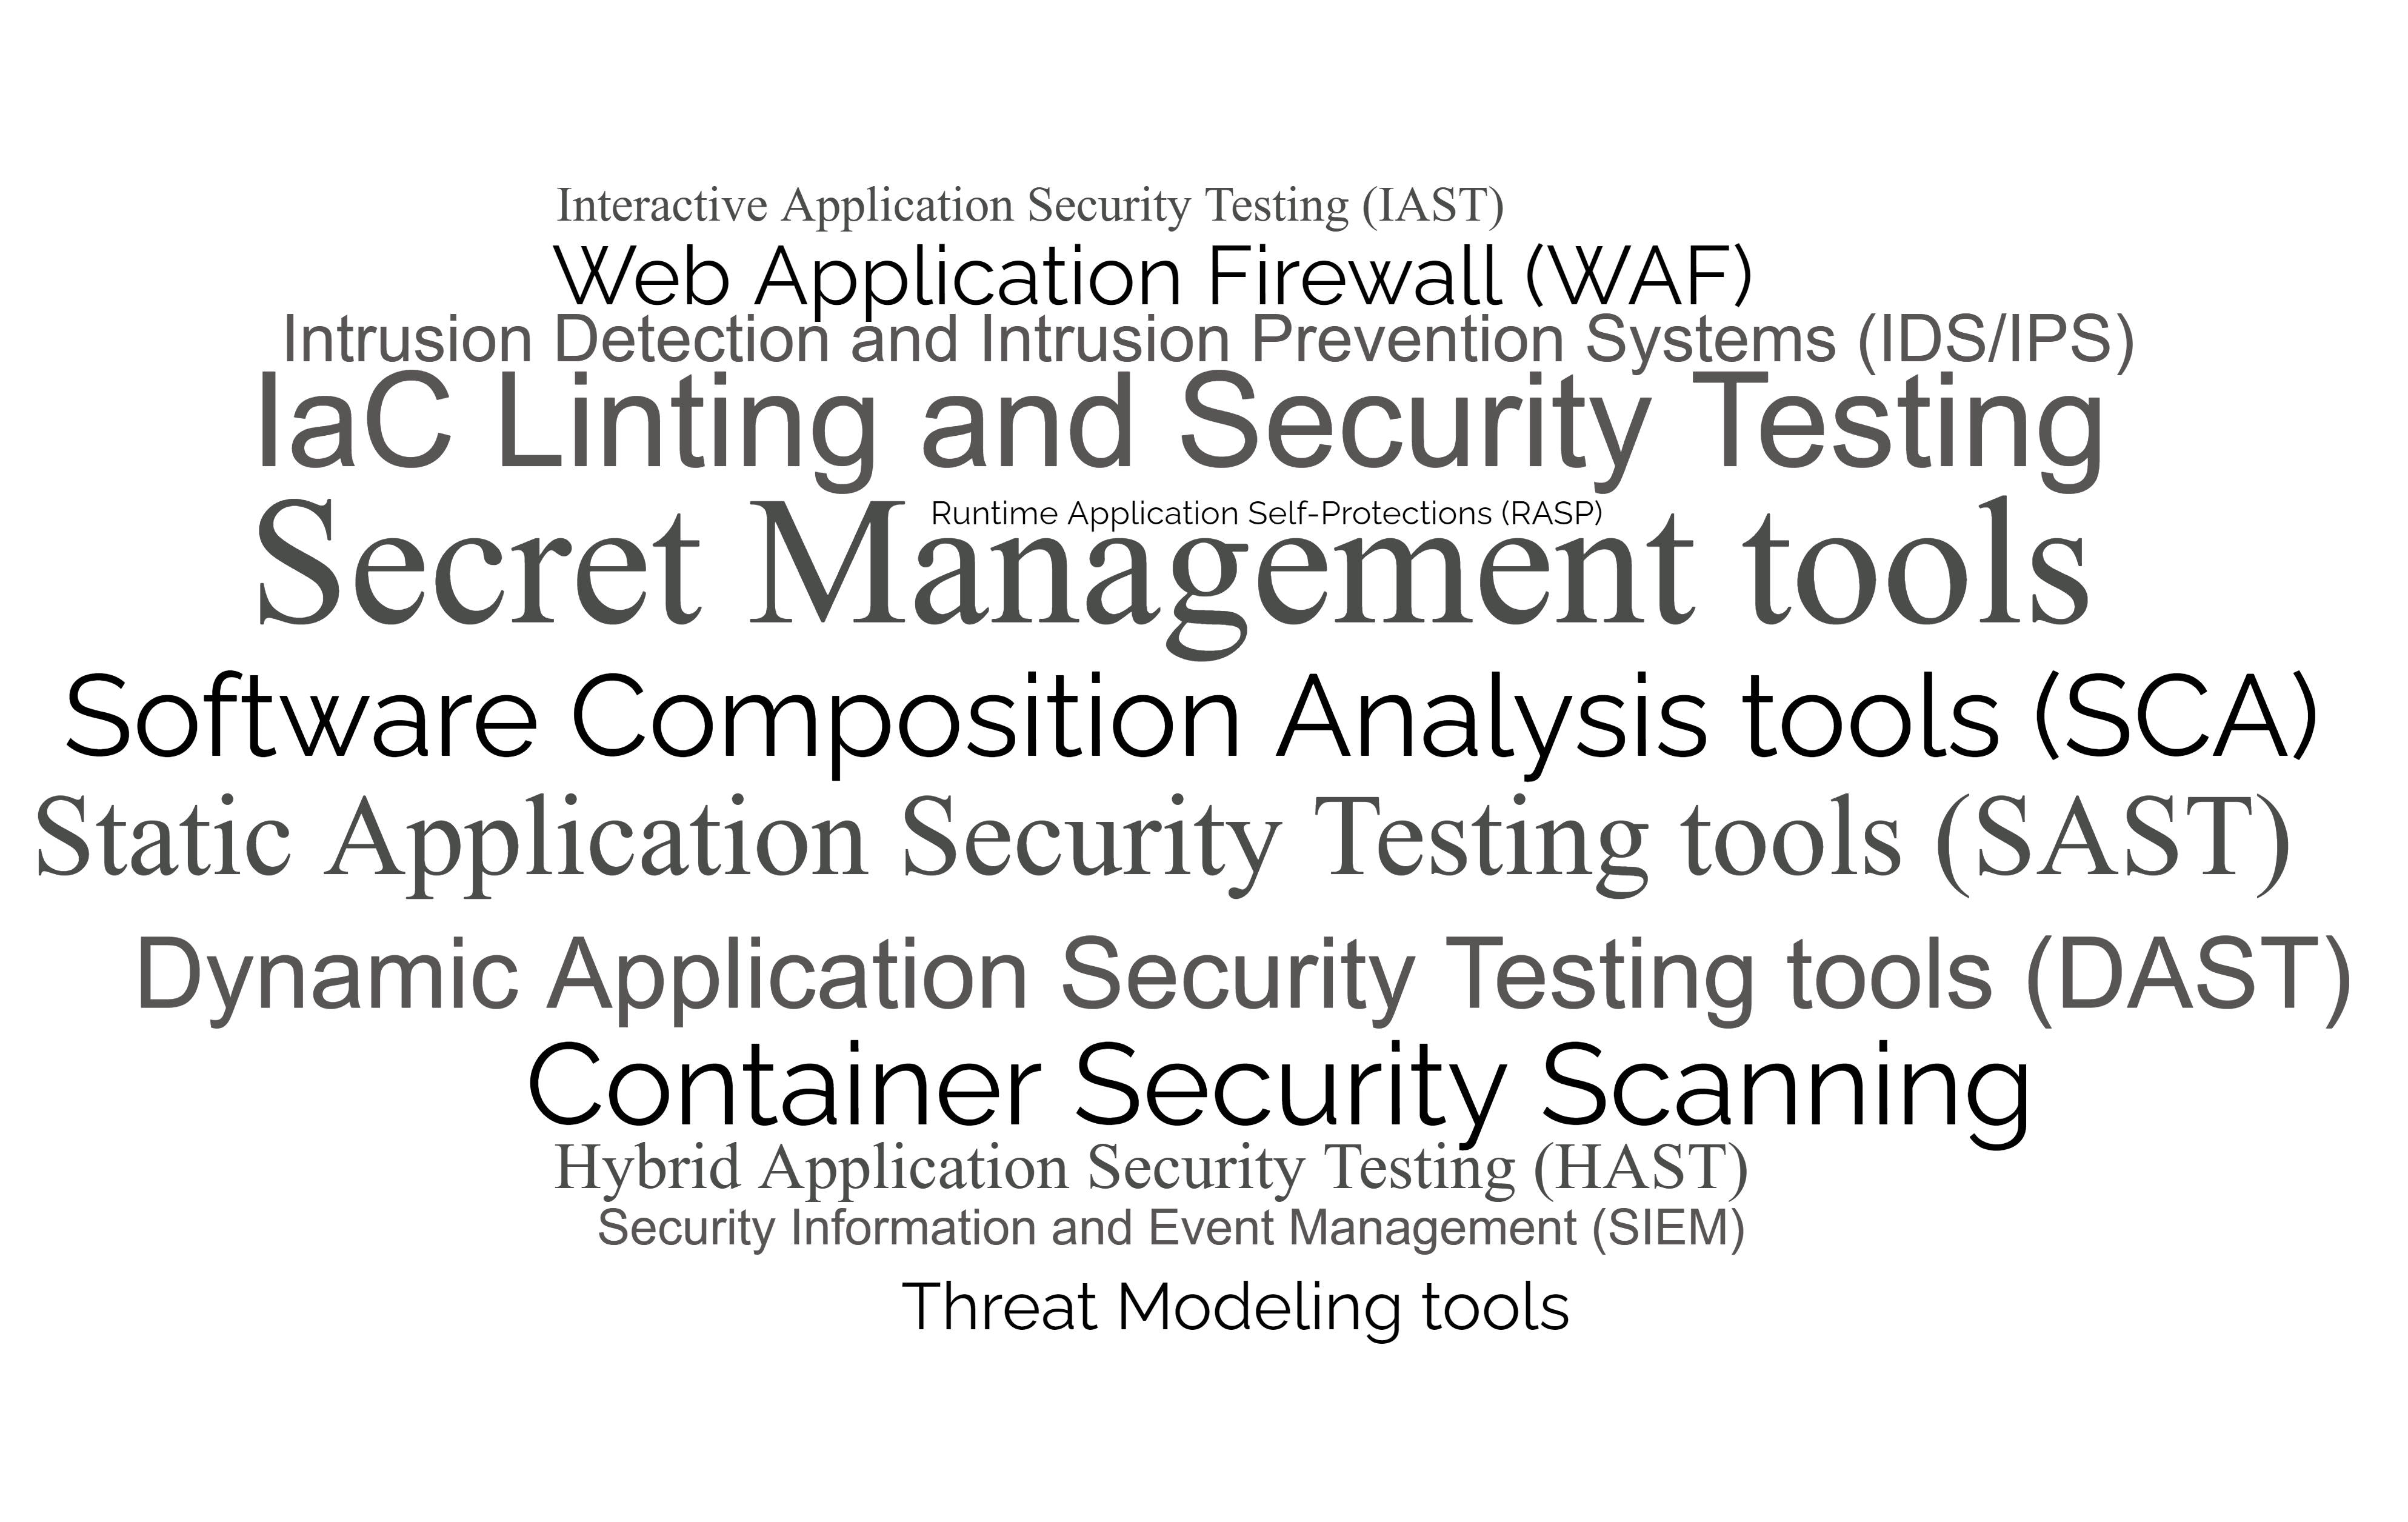
\includegraphics[scale=0.12]{graphics/wordcloud.png}
  \caption{\label{fig:wordcloud}Verschillende categorieën van tools \autocite{Martelleur2022}}
\end{figure}
\clearpage

\textcite{Martelleur2022} beschrijven welke tools het meest gebruikt worden binnen DevSecOps en wat de sterktes en zwaktes zijn van deze tools. Statisch applicatie security testing (SAST) tools bijvoobeeld zijn vatbaar voor veel valse positieven wat leidt tot foutieve resultaten. Dynamische applicatie security testing tools daarentegen zijn moeilijk om op een correcte wijze op te zetten en er is veel tijd nodig om correcte resultaten te verkrijgen. In het onderzoek worden ook enkele algemene opmerkingen over de tools aangehaald.

% nog toevoegen van definites sast en dast met eigen woorden

\begin{itemize}
  \item Er is onvoldoende documentatie om de tools op een correcte manier op te zetten.
  \item Verschillende tools zijn niet aangepast om gebruikt te worden in een DevSecOps omgeving.
  \item Tools kunnen soms moeilijk geïntegreerd worden in de deploy fase.
  \item Door verschillende tools te gebruiken bij verschillende teams kan dit leiden tot moeilijkheden bij de samenwerking.
\end{itemize}
  
De keuze of een tool gebruikt zal worden of niet, hangt af van veel factoren. Bovenstaande factoren spelen een rol, maar er zijn nog andere factoren die bepalen of een tool in gebruik wordt genomen. \textcite{Rajapakse2022} spreken over nog drie andere redenen die bepalen of een tool geadopteerd wordt binnen de omgeving.

\begin{itemize}
  \item Er wordt gesproken over wrijving die kan ontstaan binnen het team, maar ook wrijving tussen de verschillende vakgebieden zoals de developers en mensen die bezig zijn met security.
  \item De infrastructuur is een ander punt waar rekening mee gehouden moet worden. Sommige omgevingen zijn te complex en zijn niet voorzien van de juiste middelen om bepaalde tools te integreren in de omgeving.
  \item De menselijke factor speelt ook een rol wanneer er gesproken wordt over DevSecOps. Niet iedereen beschikt over de nodige vaardigheden om security op de juiste manier te implementeren. Interne strubbelingen binnenin een team is een ander voorbeeld van een menselijke oorzaak die tot het falen kan leiden.
\end{itemize}

Hoe effectief deze hulpmiddelen zijn bij het vinden van kwetsbaarheden in applicaties en bijgevolg secrets wordt, door \textcite{Thulin2015} besproken in zijn master thesis. Vaak is er een combinatie van verschillende tools nodig om tot het beste resultaat te komen. SAST tools volstaan bij de meeste scenario's niet als security middel. Door het toevoegen van dynamische tools en door analyses uit te voeren tijdens de runtime van de applicatie, kan een beter resultaat verkregen worden. 

\subsection{\IfLanguageName{dutch}{DevSecOps tools om secrets te herkennen en beheren}{DevSecOps tools to recognize and manage secrets}}
\label{sec:DevSecOps tools om secrets te herkennen en beheren}

Wanneer er gesproken wordt over het foutief gebruik van secrets, is het echter een ander verhaal. Het is zeer moeilijk om te detecteren wat als een secret beschouwd kan worden in een bepaalde context. Bijgevolg zijn er dus heel wat valse positieven wanneer gebruik wordt gemaakt van klassieke methodes. Met de komst van machine learning (ML) algoritmes kunnen secrets zoals wachtwoorden, API-sleutels, certificaten en andere vormen van vertrouwelijke gegevens sneller herkend worden. Aan de hand van patronen en veel gebruikte formaten is het mogelijk om het model aan te leren hoe een secret er precies uit ziet. Op die manier is het dus veel efficiënter geworden om gevoelige informatie te herkennen \autocite{Saha2020}.

\section{\IfLanguageName{dutch}{Kwetsbaarheden en aanvallen om secrets te extraheren}{Vulnerabilities and attacks to extract secrets}}%
\label{sec:Kwetsbaarheden en aanvallen om secrets te extraheren}

\subsection{\IfLanguageName{dutch}{Secret Sprawl}{Secret Sprawl}}
\label{sec:Secret Sprawl}
Waarom het vaak nog altijd zeer eenvoudig is om gevoelige informatie te vinden kan geïllustreerd worden met een report van \Textcite{GitGuardian2021}. Dit bedrijf ontwikkelde een tool om secrets zoals API keys, security certificaten en wachtwoorden te detecteren in GitHub repositories. In hun 2021 rapport werd beschreven hoeveel secrets er nog altijd te vinden zijn online. Meestal is het niet de bedoeling dat de developer deze geheime informatie beschikbaar stelt.

\begin{itemize}
  \item Wanneer er gebruik wordt gemaakt van een versiebeheer systeem echter, is het eenvoudig dit systeem foutief te configureren.
  \item Ook worden alle secrets bewaard in de versiegeschiedenis van dit systeem en is deze informatie dus publiekelijk beschikbaar.
  \item Doordat er steeds meer een tendens is naar het encrypteren van secrets en bijgevolg het minder toegankelijk maken van deze informatie, kan het gebeuren dat de developer kiest om deze gegevens te hard coderen en op een onveilige manier te distribueren.
  \item Er zijn ook steeds meer secrets omdat er veel meer gebruik wordt gemaakt van cloud technologieën en er is gewoon meer informatie die beschermd moet worden.
\end{itemize}
Een combinatie van deze factoren leidt tot een concept dat "Secret Sprawl" genoemd wordt \autocite{GitGuardian2021}.
\clearpage


\subsection{\IfLanguageName{dutch}{Bedreigingen in de pipeline}{Threats in the pipeline}}
\label{sec:Bedreigingen in de pipeline}
Als een aanvaller wil binnen dringen in de pipeline moet hij vaak niet ver zoeken. "Secret Sprawl" en het slordig gebruik van gevoelige informatie zorgt ervoor dat hij al snel toegang verkrijgt tot de belangrijkste componenten van de omgeving. Op die manier kan de aanvaller de omgeving compromitteren in slechts enkele minuten \autocite{Smart2022}. Er is heel wat onderzoek verricht naar de verschillende bedreigingen die voorkomen binnen de pipeline. \textcite{Rimba2015} beschrijft hoe er door het gebruik van security patronen\footnote{Een beveiligingspatroon vertegenwoordigt een gedefinieerde en herbruikbare oplossing voor een terugkerend beveiligingsprobleem. (Verkregen maart 31, 2023, van \url{https://securitypatterns.io/docs/how-to-write-a-security-pattern/})} een veiligere pipeline gecreëerd kan worden. In deze paper worden er ook een aantal risico’s aangehaald die kunnen leiden tot het misbruik van de CI/CD omgeving.
 
\begin{itemize}
  \item Secrets die publiekelijk beschikbaar zijn en op die manier krijgt men toegang tot de pipeline.
  \item Als gebruiker toegang hebben tot bepaalde code repositories die gebruikt worden binnen de pipeline.
\end{itemize}

In ander onderzoek van \textcite{Ullah2017} worden er nog andere risico's aangehaald.

\begin{itemize}
  \item Code injectie door het falen van de security.
  \item Onvoldoende toegangscontrole voorzien in de buildserver.
\end{itemize}

\textcite{Ullah2017} wijst erop dat elke component die deelneemt aan de pipeline evenveel aandacht zou moeten krijgen op vlak van beveiliging. Het toevoegen van authenticatie middelen bijvoorbeeld, is een eerste stap om een extra beveiligingslaag te creëren.
\newline

Om een gedetailleerdere lijst van bedreigingen op te stellen kan er gebruik worden gemaakt van een threat model zoals STRIDE. \textit{\textbf{STRIDE} wordt gebruikt om security bedreigingen in kaart te brengen. Deze bedreigingen worden geclassifiseerd volgens enkele belangrijke categorieën, deze categorieën kunnen worden teruggevonden in figuur \ref{fig:acronymSTRIDE} \autocite{VanLanduyt2021}. Binnen dit model wordt gebruik gemaakt van shift-left security. Wanneer een shift-left aanpak gevolgd wordt, worden beveiligingsproblemen zo vroeg mogelijk in de ontwikkeling fase aanpakt. \autocite{Kantor2021}"} \textcite{Paule2018} beschrijft in zijn master thesis hoe het STRIDE-model gebruikt om de belangrijkste bedreigingen te detecteren. Deze bedreigingen worden vervolgens gekoppeld aan mogelijke kwetsbaarheden. Door gebruik te maken van dit model kunnen de bedreigingen geclassificeerd worden volgens het type aanval. 
\newline

In het onderzoek van \textcite{Paule2018} wordt ook aangehaald dat niet enkel de componenten van de pipeline kwetsbaar zijn, maar ook de verschillende artefacten\footnote{Een artefact is een bijproduct van softwareontwikkeling. Het is alles wat ontstaat wanneer een stuk software ontwikkeld wordt (Verkregen maart 31, 2023, van \url{https://artifacts.ai/what-is-an-artifact/})} die ontstaan wanneer de pipeline uitgevoerd wordt.

\begin{figure}[H]
  \centering
  \begin{itemize}
    \setlength\itemsep{0.1em}
    \item\textbf{S}poofing
    \item\textbf{T}ampering
    \item\textbf{R}epudiation
    \item\textbf{I}nformation Disclosure
    \item\textbf{D}enial of Service
    \item\textbf{E}levation of Privilege
    \caption{\label{fig:acronymSTRIDE}Uitleg over het acroniem STRIDE (Verkregen maart 31, 2023, van \url{https://threat-modeling.com/stride-threat-modeling/})}
  \end{itemize}
\end{figure}

\subsection{\IfLanguageName{dutch}{Aanvallen binnenin pipeline}{Attacks in the pipeline}}
\label{sec:Aanvallen binnenin pipeline}
\textcite{Pecka2022} tonen aan dat wanneer toegang verkregen wordt tot de CI/CD pipeline, het zeer eenvoudig is om geheime informatie op te halen voor bijvoorbeeld een Kubernetes cluster. Het is dan ook niet meer moeilijk om binnen te dringen in de achterliggende infrastructuur. Niet alleen de pipeline is een doelwit voor aanvallers, alle componenten die deelnemen en een invloed uitoefenen op de pipeline zijn interessante doelwitten.
\newline

\textcite{Security2022} beschrijven hoe het mogelijk is omgevingsvariabelen uit te lezen via een Poisened Pipeline Execution (PPE) aanval. {\centering\textit{"\textbf{PPE aanvallen} verwijzen naar het vermogen van een aanvaller met toegang tot broncontrolesystemen – en zonder toegang tot de bouwomgeving, om het bouwproces te manipuleren door kwaadaardige code/commando's in de configuratie van de build pipeline te injecteren, in feite de pipeline te 'vergiftigen' en kwaadaardige code uit te voeren als onderdeel van het bouwproces \autocite{Security2022}."}}
\newline

Een PPE aanval kan volgende drie vormen aannemen. \textbf{Directe PPE (D-PPE)} komt voor wanneer de aanvaller de CI configuratie file kan herschrijven en via een pull request de build kan beïnvloeden. Wanneer de threat actor niet rechtstreeks toegang heeft tot de de CI configuratie file kan hij nog steeds het bouw proces beïnvloeden. Hij maakt bij deze vorm van PPE gebruik van de bestanden waar naar gerefereerd wordt in de pipeline. Deze vorm van PPE wordt \textbf{indirecte PPE (I-PPE)} genoemd. Een derde en laatste vorm is \textbf{Publieke PPE of (3PE)}. Er wordt gesproken van 3PE wanneer de CI configuratie file publiekelijk gehost wordt en de aanvaller hier gebruik van maakt.
\newline

In het report van \textcite{Security2022} worden ook nog enkele andere soorten aanvallen besproken. Doordat er soms wel gebruik wordt gemaakt van 3rd party elementen in een pipeline wordt het aanval oppervlak vergroot. In deze aanvallen zijn de verschillende onderdelen van de omgeving het doelwit. Het misbruiken van "dependencies" en het misbruiken van plugins die gebruikt worden binnenin de pipeline scripts zijn slechts enkele aanvallen die tot deze categorie behoren. Sommige plugins die beschikbaar zijn voor Jenkins zijn vaak niet duidelijk omschreven. Wanneer deze plugins gebruikt worden in een omgeving en deze zijn dus fout geconfigureerd, leidt dit tot een ander toegangspunt voor de aanvaller. \autocite{Haymore2022} omschrijven in een artikel van NCC Group verschillende aanvallen die mogelijk zijn wanneer op een incorrecte manier gebruik gemaakt wordt van een specifieke technologie. Een Amazon S3 bucket bijvoorbeeld wordt gebruikt om gegevens op te slaan, maar als deze fout geconfigureerd is, is dit het perfect toegangspunt voor de aanvaller. 

\subsection{\IfLanguageName{dutch}{Praktische voorbeelden van pipeline aanvallen uit de security wereld}{Practical examples of pipeline attacks from the security scene}}
\label{sec:Praktische voorbeelden uit de securitywereld}
Doordat de CI/CD oplossing GitLab gebruik maakt van runners\footnote{GitLab Runner is een applicatie die samenwerkt met de GitLab CI/CD pipeline om jobs in een pipeline uit te voeren. Deze applicaties kunnen zelf beheerd worden of er kan geopteerd worden voor een runner die door GitLab beheerd wordt. (Verkregen maart 31, 2023, van \url{https://docs.gitlab.com/runner/})} worden er nieuwe kwetsbaarheden geïntroduceerd. \textcite{Haymore2022} beschrijven hoe een GitLab pipeline misbruikt kan worden door gebruik te maken van deze foutief geconfigureerde runners. De meeste aanvallen in deze omgevingen ontstaan doordat componenten in GitLab vaak voorzien zijn van te veel rechten, bijvoorbeeld Docker containers die uitgevoerd worden met de verkeerde rechten. Door gebruik te maken van deze rechten kan de aanvaller ontsnappen uit de Docker omgeving en op die manier zijn privileges escaleren. Deze runners kunnen ook misbruikt worden om secrets te extraheren omdat de CI/CD jobs niet genoeg beveiligd zijn en door de repositories die gebruikt worden in deze jobs. Een aanval binnen de pipeline kan heel divers zijn en toont aan dat het "attack surface" van een CI/CD omgeving heel groot kan worden.
\clearpage

Op het evenement \href{https://www.blackhat.com/us-22/}{Black Hat USA 2022} verklaarden \textcite{Smart2022} waarom het van cruciaal belang is dat er op een correcte manier omgegaan wordt met secrets. Bij hun aanvallen op de CI/CD pipelines, komen zij vaak het eerst in aanraking met secrets en daardoor is het zeer eenvoudig toegang te verkrijgen tot de achterliggende software. Verschillende aanvallen zijn niet alleen te danken aan het slordig gebruik van secrets, maar ook het niet toepassen van least privilege Roll Based Access Control (RBAC). Doordat de aanvaller zich voordoet als legitieme bron en doordat hij misbruik maakt van incorrecte configuraties, is het kinderspel voor hem om binnen te breken in een CI/CD omgeving.
\newline

De soort pipeline die gebruikt wordt kan ook problemen veroorzaken. Uit een onderzoek van \textcite{Koishybayev2022} blijkt dat bepaalde CI/CD software niet over voldoende beschermingsmaatregelen beschikken om een veilige pipeline te kunnen garanderen. Geheime informatie kan lekken doordat deze in de logs beschikbaar is. Er wordt aangehaald dat enkel de plugins en stappen waar de secrets gebruikt worden toegang mogen hebben tot de geheime informatie. Anders is deze informatie beschikbaar voor alle componenten in het systeem, wat tot beveiligingsrisico's kan leiden.
\newline 

De software die dagelijks gebruikt wordt in een CI/CD omgeving is een ander kwetsbaar punt. Zeer recent was er een kwetsbaarheid in TerraForm waardoor Remote Code Execution (RCE) mogelijk was. {\centering\textit{"\textbf{Remote code execution (RCE)} verwijst naar een klasse van cyberaanvallen waarbij aanvallers op afstand opdrachten uitvoeren om malware of andere kwaadaardige code op een computer of netwerk te plaatsen. Bij een RCE-aanval is er geen gebruikersinput nodig \textcite{Baker2021}."}} \textcite{Suezawa2021} en, \textcite{Kaskasoli2021} en, \textcite{Frank2021} spreken allemaal over de aanval die mogelijk was wanneer gebruik werd gemaakt van Terraform. Op \href{https://defcon.org/html/defcon-29/dc-29-index.html}{DEFCON 29} toont \textcite{Ahmed2021} aan dat er nog andere manieren zijn om deze omgeving aan te tasten. De Terrform API is kwetsbaar omdat er gevoelige informatie opgehaald kan worden. Via deze API is het mogelijk Terraform state files op te halen en deze files kunnen “cleartext” secrets bevatten. {\centering\textit{"\textbf{Terraform state files} zijn json bestanden waarin de omgeving die met terraform is opgezet is beschreven. Deze bestanden geven een overzicht van de volledige infrastructuur die is opgezet \autocite{Salecha2023}."}} Providers waar gebruik van wordt gemaakt binnen de build scripts in de Terraform omgeving, kunnen gecompromitteerd zijn en op die manier kan een achterpoort ingebouwd worden in de pipeline.
\clearpage

Infrastructure as code (IAC) is een andere punt langs waar een aanval mogelijk is. \textit{"\textbf{Infrastructuur als code} houdt in, het beheren en aanbieden van infrastructuur als code. De infrastructuur wordt voorzien aan de hand van configuratie bestanden. Op die manier kan infrastructuur sneller opgezet worden en is het beheren van deze infrastructuur veel gemakkelijker. \autocite{Huettermann2012}."} Figuur \ref{fig:IACAttack} toont een voorbeeld van hoe deze aanval in zijn werk kan gaan. \textcite{Suezawa} beschrijft in zijn presentatie voor \href{https://codeblue.jp/2021/en/}{CODE BLUE 2021 OpenTalks} hoe een hacker de Cloud infrastructuur kan binnendringen door gebruik te maken van IAC-functionaliteiten. In DEFCON 29 toont \textcite{Bar2021} aan dat zelf de SAST en DAST tools die gebruikt worden om de security van applicaties te testen, kwetsbaarheden bevatten. Meeste van deze kwetsbaarheden leiden tot RCE, maar sommige kunnen ook andere aanvallen veroorzaken zoals denial of service (DOS) aanvallen. \textit{"Een DOS aanval is een aanval waarbij de aanvaller probeert om een network, systeem of toepassing te overbelasten. Op die manier hebben de gebruikers van het systeem geen toegang meer tot de service \autocite{LenaertsBergmans2023}."} Vooraleer tools gebruikt worden in het development proces en dus de pipeline, is het belangrijk dat het security team nadenkt hoe deze tools misbruikt kunnen worden.

\begin{figure}[H]
  \centering
  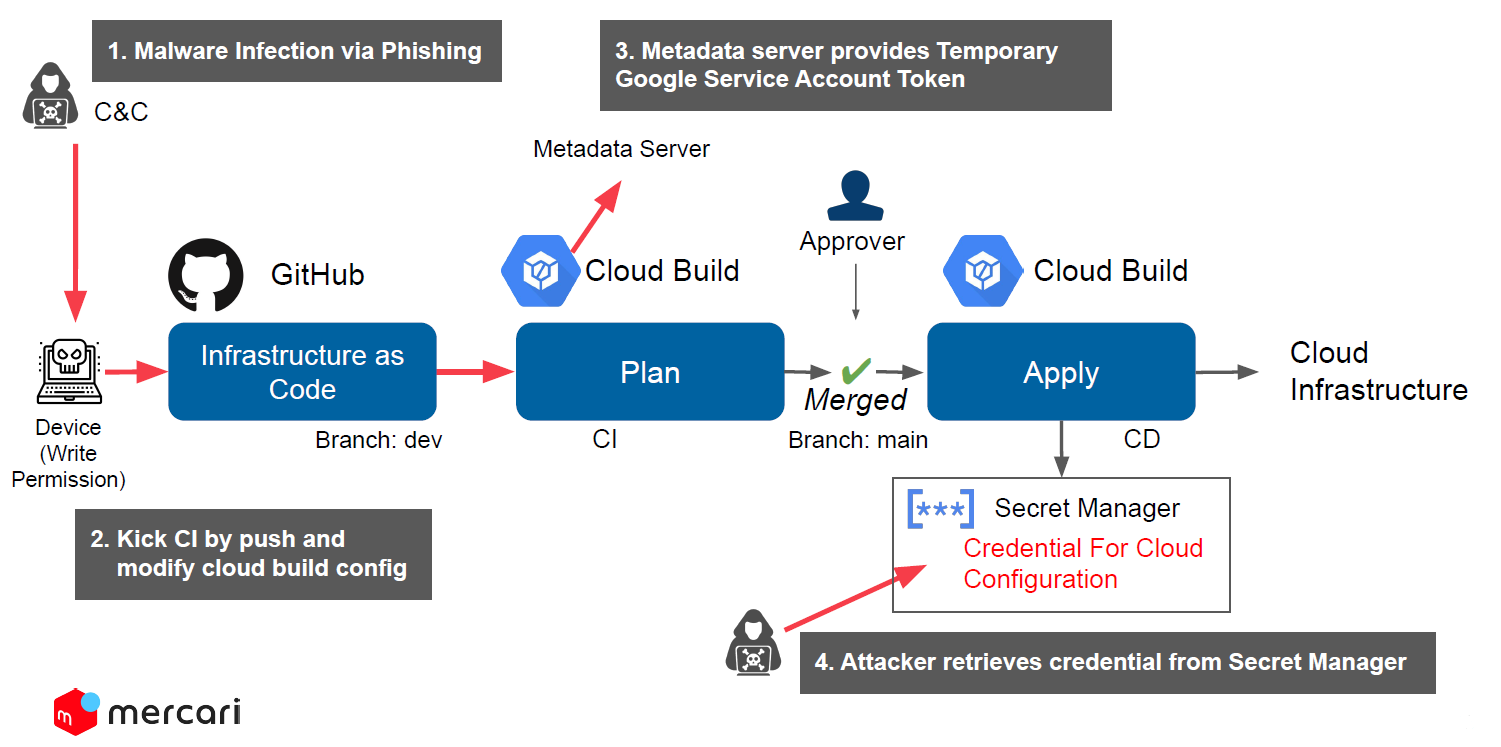
\includegraphics[scale=0.38]{graphics/IACAttack.png}
  \caption{\label{fig:IACAttack}Aanval op de pipeline via IAC \autocite{Suezawa2021}}
\end{figure}

\section{\IfLanguageName{dutch}{Beveiligingsmaatregelen om secrets te beschermen}{Security measures to protect secrets}}
\label{sec:Beveiligingsmaatregelen om secrets te beschermen}

\subsection{\IfLanguageName{dutch}{Secrets in versie beheer en basis security principes}{Secrets in version control and basic security principles}}%
\label{sec:Secrets in versie beheer en basis security principes}
De eerste stap om aanvallen op de pipeline te verhelpen ligt bij het volgen van de basis security principes, \autocite{Smart2022} en,  \autocite{Haymore2022} en, \autocite{Suezawa2021} halen deze principes in hun onderzoek steeds terug aan. Figuur \ref{fig:wordcloudv2} toont een overzicht van deze security principes. 
\clearpage 

\begin{figure}[H]
  \centering
  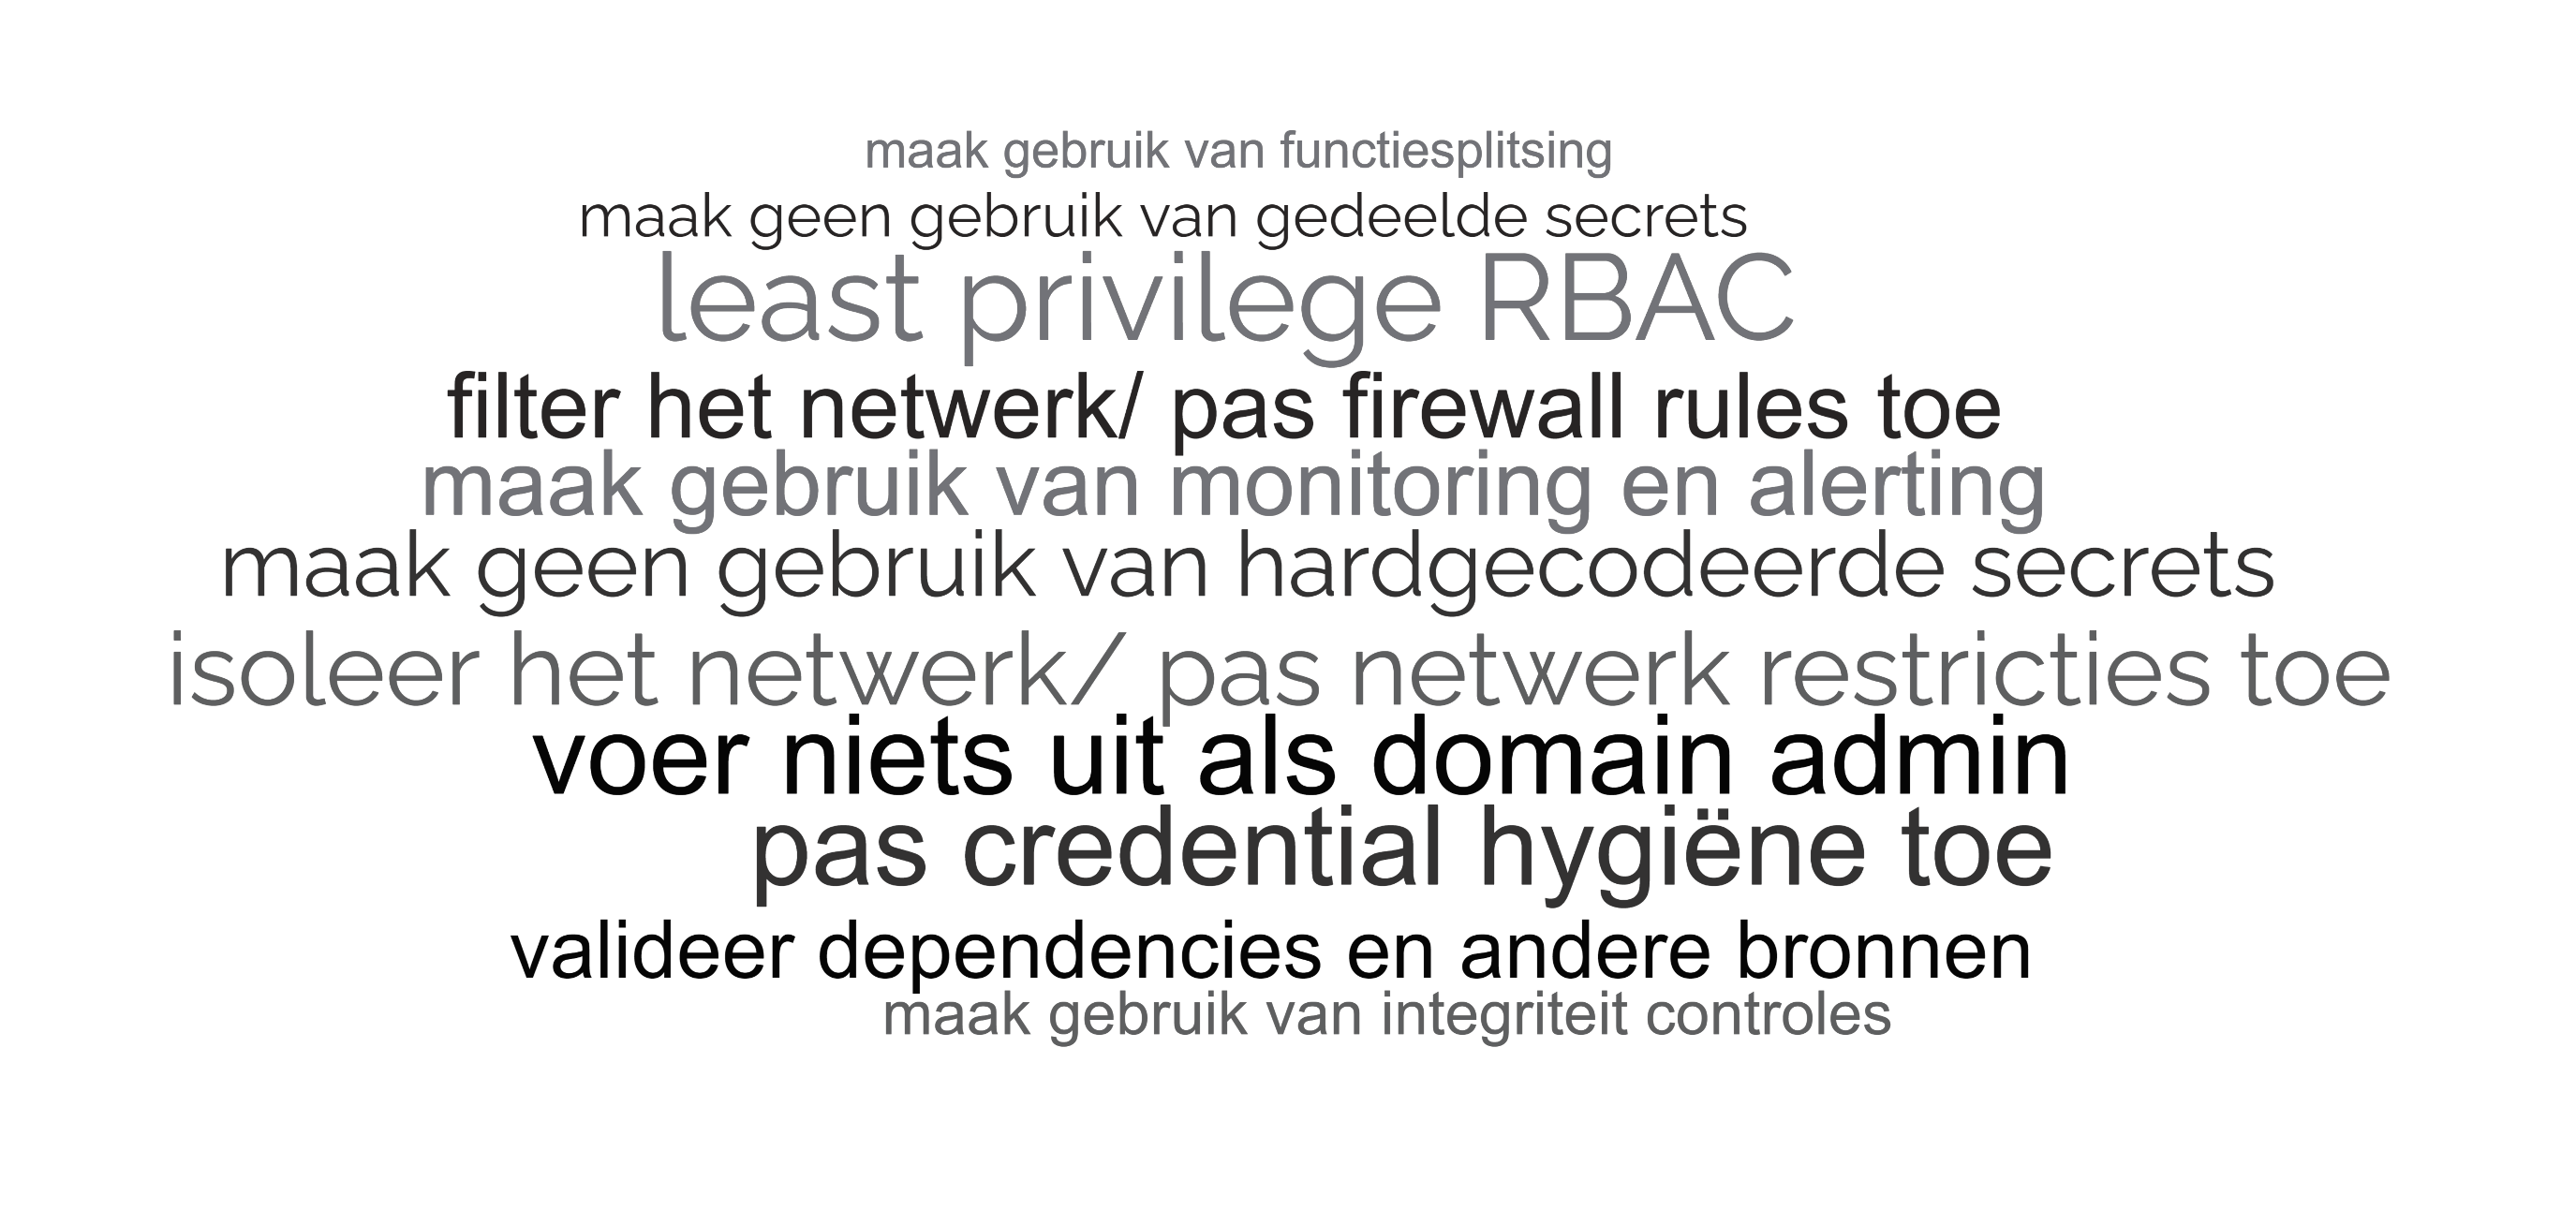
\includegraphics[scale=0.14]{graphics/wordcloudv2.png}
  \caption{\label{fig:wordcloudv2}Verschillende basis security principes \autocite{Smart2022} en, \autocite{Haymore2022} en, \autocite{Suezawa2021}}
\end{figure}


Vooraleer de secrets gebruikt zullen worden bij de bouw van de infrastructuur of applicaties, is het belangrijk dat de versie beheersystemen (VCS) van de nodige veiligheidsmaatregelen voorzien zijn. Als deze systemen niet voldoende beveiligd zijn kan de threat actor binnendringen in slechts enkele minuten. In het onderzoek van \autocite{Mouw2021} zijn bepaalde experimenten uitgevoerd die duidelijk vastleggen hoelang het duurt vooraleer deze systemen op iemand zijn radar verschijnen.
\newline 

In een literatuurstudie van \textcite{Basak2023} worden enkele "best practices" besproken over het gebruik van secrets in een VCS. 

\begin{itemize}
  \item Laat secrets zoveel mogelijk weg te laten uit de repositories, bewaar secrets in de plaats in configuratie bestanden.
  \item Maak gebruik van gitignore op de juiste manier.
  \item Gebruik geen private repositories om secrets te bewaren.
  \item Zorg ervoor dat wanneer er gecommit wordt naar de VCS dat er geen secrets geleaked kunnen worden.
  \item Maak gebruik van tools zoals TruffleHog, Gitrob en git-all-secrets om de VCS te scannen.
  \item Maak gebruik van git hooks en git flags bij de pre commit en post commit zodat commits tegen kunnen gehouden worden.
\end{itemize}

Indien secrets toch niet tegengehouden worden door deze maatregelen, is het belangrijk de gelekte credentials in te trekken en de VCS-geschiedenis te verwijderen. Er mag vanuit gegaan worden dat wanneer deze situatie zich voordoet, de geheime informatie gecompromitteerd is vanaf dat moment.


\subsection{\IfLanguageName{dutch}{Secrets in infrastructure as code en secrets beheer}{Secrets in infrastructure as code en secrets management}}%
\label{sec:Secrets in infrastructure as code en secrets beheer}
CI/CD pipelines worden niet enkel gebruikt om applicaties te bouwen, een groot deel van deze pipelines is gereserveerd voor het opbouwen van infrastructuur. Deze infrastructuur wordt opgebouwd aan de hand van code en is een andere component van de CI/CD omgeving waar rekening mee gehouden moet worden. Veel van deze IAC-scripts bevatten te veel hard gecodeerde secrets. Gebruikers maken niet op de juiste manier gebruik van de ingebouwde tools die beschikbaar zijn om de secrets te beschermen \autocite{Rahman2019},\autocite{Kumara2021}.
\newline

\textcite{Morris2021} bespreekt in zijn boek verschillende manieren om secrets te beschermen binnen de IAC wereld. Encryptie van secrets, autorisatie zonder secrets, injectie van secrets tijdens runtime en wegwerpbare secrets zijn enkele initiatieven die genomen kunnen worden om een veiligere IAC-omgeving te creëren. In het onderzoek van \textcite{Rahman2021} wordt uitgebreider ingegaan op deze categorieën en worden ook nog enkele andere belangrijke beveiligingsmaatregelen besproken.

\begin{itemize}
  \item Pas niet zomaar encryptie toe op alle gegevens, ga na welke belangrijk zijn en prioriteit krijgen.
  \item Wanneer autorisatie zonder secrets geen mogelijkheid is implementeer het juiste toegangscontrole beleid.
  \item Maak gebruik van RBAC wanneer toegangscontrole geïmplementeerd wordt.
  \item Houd artefacten gescheiden wanneer mogelijk.
  \item Log alle operaties die gebeuren in verband met secrets binnen de IAC-scripts.
  \item Roteer secrets zoveel mogelijk.
\end{itemize}

Zoals al eerder aangehaald werd in een inleidende paragraaf,zijn scanning tools een extra maatregel die kunnen helpen in de strijd tegen de cybercriminelen. CredScan en SLIC zijn voorbeelden van scanners voor de IAC-omgeving.\autocite{Rahman2021} 
\newline

Om heel wat problemen te vermijden is het nog altijd de optie om secrets in een kluis\footnote{HashiCorp Vault, AWS Secret Manager, Cloud KMS, Microsoft Azure Key Vault.} te bewaren. Deze opslagplaatsen zijn voorzien van de meeste van de opgesomde maatregelen en maken het beheer van al deze informatie veel eenvoudiger. Ook zorgen deze tools ervoor dat de secrets niet zichtbaar zijn in de logs of de shell geschiedenis \autocite{Agarwal2021}. 
\clearpage

Verschillende onderzoekers documenteerden al eerder hoe er best omgegaan wordt met secrets. In de paper van \autocite{Basak2023} wordt advies gegeven in verband met het gebruik en de bescherming van secrets. Het advies dat gegeven wordt in dit onderzoek is zeer gelijkaardig aan hetgeen eerder vermeld werd in verband met IAC scripts. Dit advies bevat echter, ook een aantal nieuwe oplossingen om secrets te beschermen.

\begin{itemize}
  \item Gebruiken van environment variabelen tijdens runtime.
  \item Inladen van secrets via een extern systeem.
  \item Vermijd het gebruik van secrets in client-side applicaties door web service functionaliteiten toe te voegen.
  \item Voorzie de API's die gebruikt worden om secrets op te halen van de correcte permissies en beperk toegang zoveel mogelijk.
\end{itemize}

Secrets in de pipeline worden gebruikt in de verschillende fasen van de pipeline zoals te zien is op figuur \ref{fig:Pipelinesecrets} Het is belangrijk maatregelen te voorzien voor al deze fases. Secrets in rust kunnen geëncrypteerd worden en beschermd worden door middel van secret managementsoftware. Secrets in de gebruiksfase worden ook beste beschermd op dezelfde manier. Daarnaast door de development, test en productomgeving te scheiden worden deze secrets extra beschermd.\autocite{Basak2022} In het boek \textcite{Calles2020} wordt het secrets verhaal meer vanuit een business perspectief bekeken. De "best practices" besproken in dit boek leunen sterk aan bij de voorgaande, maar er wordt ook besproken hoe de Cloud gebruikt kan worden om secrets te managen. Amazon, Google, Microsoft hebben allemaal een key management systeem, waardoor secrets in de Cloud op een veilige manier gebruikt kunnen worden.

\begin{figure}[H]
  \centering
  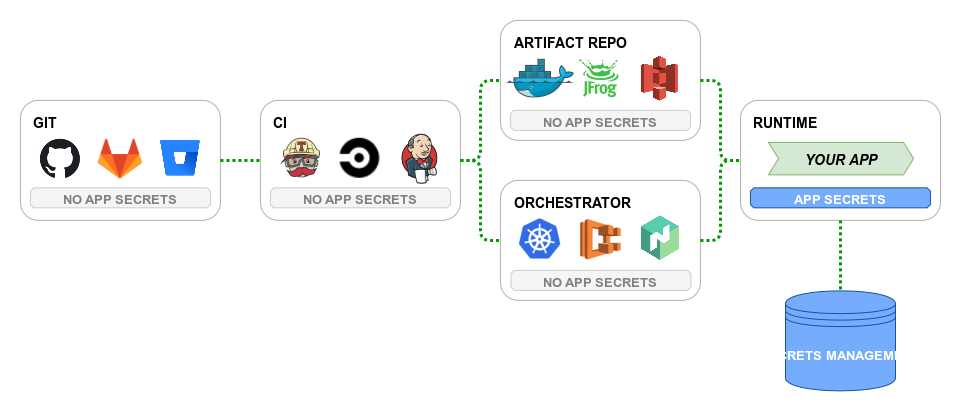
\includegraphics[scale=0.4]{graphics/Pipelinesecrets.png}
  \caption{\label{fig:Pipelinesecrets}Gebruik van secrets doorheen de pipeline (Verkregen maart 31, 2023, van \url{https://secrethub.io/blog/decouple-application-secrets-from-ci-cd-pipeline/})}
\end{figure}

% boeken pagina’s en hoofdstuk vermelden
\subsection{\IfLanguageName{dutch}{Beheer van secrets in containers}{Management of secrets in containers}}%
\label{sec:Beheer van secrets in containers}
Containers worden steeds meer gebruikt bij het bouwen van software. Een container is een bundel van data die elk element bevat die nodig is om een applicatie uit te voeren. Deze bundel bevat de applicatie code, libraries en dependencies \autocite{Levine2020}. Containers maken deel uit van de CI/CD pipelines. Het beveiligen van containers is daarom zeer belangrijk. Risico's zoals secrets die ingebakken zitten in de image kunnen opgemerkt worden met containerscanners. Wanneer deze tools secrets of andere kwetsbaarheden detecteren, is er de mogelijkheid om het bouwproces te laten falen zodat mogelijke aanvallen vermeden kunnen worden \autocite{Agarwal2021}. 


\subsection{\IfLanguageName{dutch}{Beheer van de pipeline en opstellen van security frameworks aan de hand van een bedreigingsmatrix}{Management of pipeline and creation of security frameworks using a threat matrix}}%
\label{sec:Beheer van de pipeline en opstellen van security raamwerken aan de hand van een bedreigingsmatrix}
In de top 10 van CIDR \textcite{Security2022} worden naast verschillende aanvallen ook specifieke mitigatie technieken en maatregelen beschreven om de pipeline te beschermen. Heel wat van deze maatregelen zijn gebaseerd op de basis principes van security. \textcite{Suezawa2021} beschrijft in zijn presentatie ook enkele maatregelen die uitgevoerd kunnen worden op pipeline niveau. De meeste van deze maatregelen zijn gedocumenteerd in deze \href{https://github.com/rung/threat-matrix-cicd}{threat-matrix}. Bedreiging matrices en andere security frameworks voor de CI/CD omgeving zijn slechts zeer recent in ontwikkeling.
\newline


Met enkel advies is het moeilijk om een plan op te stellen. \autocite{Koopman2019AFF} beschrijven een framework dat gebruikt kan worden voor het detecteren van kwetsbaarheden en bedreigingen. Op die manier is het mogelijk een strategie uit te werken die gebruikt kan worden binnen de organisatie. Het document van CIDR \textcite{Security2022} kan een optie zijn als classificatiesysteem om beveiligingsrisico's te herkennen. Met behulp van een matrix en een framework is het realistischer om een plan van aanpak op te stellen voor het beveiligingen van de CI/CD omgeving en bijgevolg het voorkomen van een Software supply chain attack.\textit{"\textbf{Een supply chain-aanval} is een soort cyberaanval gericht op een vertrouwde leverancier die services of software aanbiedt die van vitaal belang zijn voor de supply chain. Software supply chain aanvallen injecteren kwaadaardige code in een applicatie om alle gebruikers van een app te infecteren, terwijl hardware supply chain-aanvallen fysieke componenten beschadigen voor hetzelfde doel \autocite{Koopman2019AFF}."}
\newline

\textcite{Foundation2021} beschrijven in hun document de hoofd principes die best gevolgd worden om de veiligheid van de supply chain te garanderen. Via dit document is er een duidelijk stappenplan om de pipline te beveiligen. Ook alle sub componenten die een bepaalde invloed uitoefenen op de pipeline worden beschreven in dit document. Organisaties zoals Google, Chainguard, Intel, VMware, Cloud native, Datadog, kusari, the Linux Foundation, Citi zijn bezig met het maken van een standaard om een beter security ecosysteem te creëren. \href{https://slsa.dev}{SLSA} is het framework in ontwikkeling, waar zij mee bezig zijn. Door gebruik te maken van standaarden, is het de bedoeling dat het securityverhaal van de pipeline heel wat duidelijker wordt voor bedrijven. 

test
